
\documentclass[11pt,a4paper,landscape]{article}
\usepackage{spl}
\geometry{left=1.8cm,right=1.8cm,top=2.4cm,bottom=2.0cm}
\begin{document}
\fancyhead[L]{\small Signal Processing}\fancyhead[R]{\small Curriculum and Roadmap}
\begin{center}
  {\LARGE\bfseries Aeronautics and Space Technology Club\par}
  {\Large\bfseries IIT (ISM) Dhanbad\par}\vspace{6pt}
  {\large Signal Processing Ladder: Curriculum, Theory and Hands-On Skills\par}
\end{center}
\begin{summarybox}{A Ladder of 25 Problem Statements in Signal Processing}
Each problem is a self-contained, hands-on problem statement with a synthetic dataset of known truth and pointers to real data.
Together they take a student from the first noisy sensor reading to an end-to-end transient-detection pipeline, passing
through sampling, the mathematics of signals and systems, analog and digital electronics, DSP, detection and estimation theory
and machine learning. Total estimated effort: about 390 hours.
\end{summarybox}
\section*{Roadmap}
\begin{center}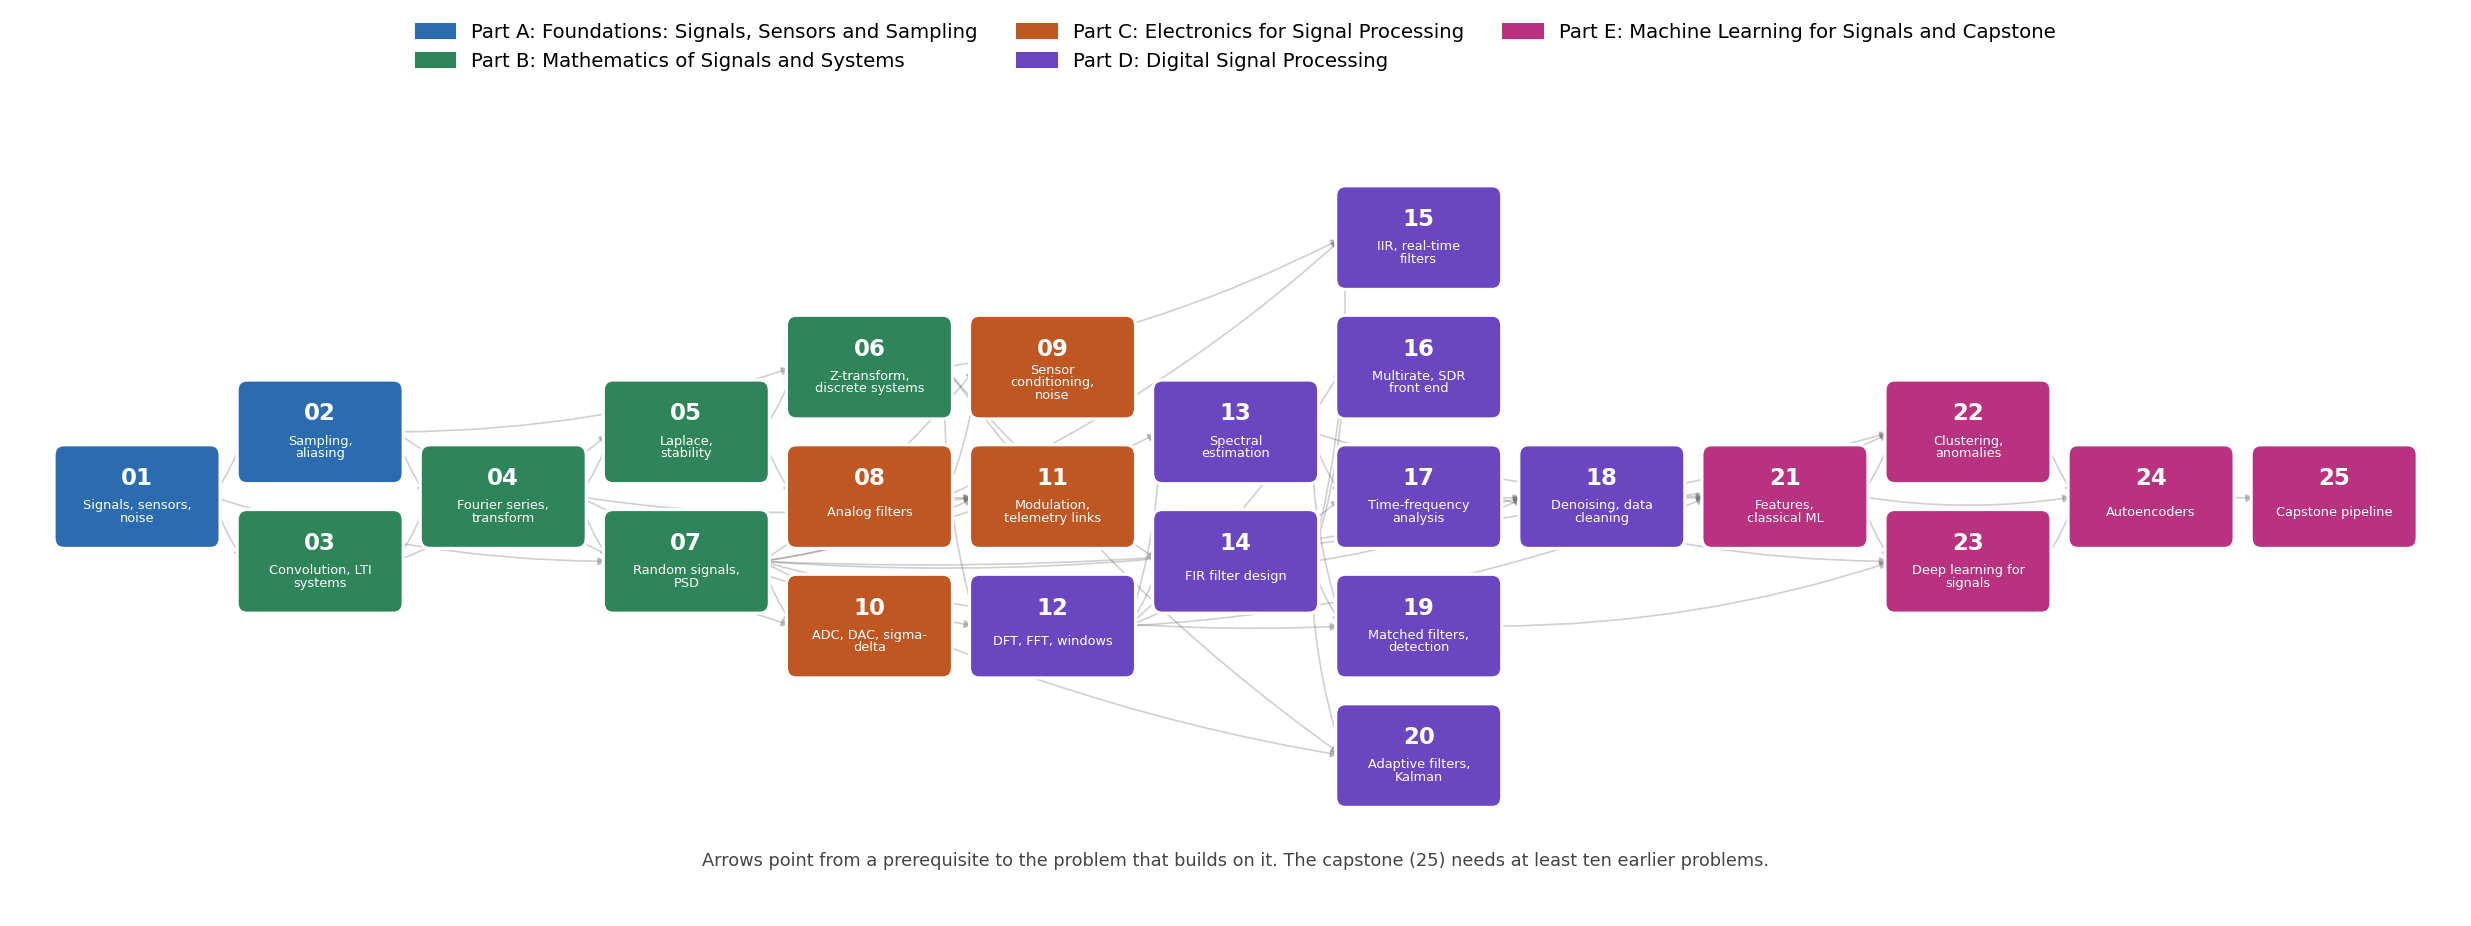
\includegraphics[width=0.98\linewidth]{images/roadmap.png}\end{center}
\section*{What You Can Do After Each Part}
\textbf{Part A: Foundations: Signals, Sensors and Sampling.} You learn to describe a signal by its power and noise, to calibrate a sensor, to separate white noise from drift with the Allan deviation, and to predict, avoid and exploit aliasing. After Part A you can look at any raw sensor stream and say how good it is and at what rate it must be sampled.\par\smallskip
\textbf{Part B: Mathematics of Signals and Systems.} You build convolution and LTI-system thinking, the Fourier transform and its uncertainty principle, the Laplace and z-transforms with pole-zero reasoning and stability, and the statistics of random signals including power spectra and Poisson counting. After Part B you can derive, not just use, the formulas of signal processing.\par\smallskip
\textbf{Part C: Electronics for Signal Processing.} You design analog filters and verify them with your own circuit solver, size a low-noise sensor front end and a lock-in detector, choose and test ADCs and DACs, and build the physical layer of a satellite telemetry link with its Doppler shift, carrier recovery and link budget.\par\smallskip
\textbf{Part D: Digital Signal Processing.} You write the FFT, understand windows and spectral scaling, estimate spectra of noise and of unevenly sampled data, design FIR and IIR filters for real-time use, resample and down-convert radio signals, analyse chirps in time and frequency, clean data without biasing it, build matched filters with calibrated false-alarm rates, and fuse sensors with adaptive filters and Kalman filters.\par\smallskip
\textbf{Part E: Machine Learning for Signals and Capstone.} You engineer features and avoid the leakage trap, detect anomalies and bursts with clustering and isolation methods, train convolutional networks and benchmark them against the optimal matched filter, build autoencoders for denoising and novelty detection, and finally assemble an end-to-end transient-detection pipeline with calibrated significance and a report.\par\smallskip
\section*{Theory and Hands-On Skills by Problem}
{\small\renewcommand{\arraystretch}{1.25}
\begin{longtable}{@{}p{0.6cm}p{3.7cm}p{8.2cm}p{7.6cm}p{2.0cm}@{}}
\toprule \textbf{\#} & \textbf{Problem} & \textbf{Theory to master} & \textbf{Hands-on skills gained} & \textbf{Effort}\\\midrule
\endhead
01 & \textbf{Signals, Sensors and Noise} & Signal classes and measures (energy, power, RMS), decibels, sensor model, noise sources, averaging, Allan variance & NumPy array handling, least-squares calibration, robust statistics, Allan deviation, reading a datasheet noise figure & 8--12 hours\\\midrule
02 & \textbf{Sampling, Aliasing and Reconstruction} & Impulse sampling, spectral replication, Nyquist theorem, aliasing, sinc reconstruction, zero-order hold, bandpass sampling, aperture jitter & Dense-grid simulation of analog signals, alias prediction, interpolation, anti-alias filter selection, jitter Monte Carlo & 8--12 hours\\\midrule
03 & \textbf{Complex Numbers, Convolution and LTI Systems} & Complex exponentials and phasors, linearity and time invariance, impulse response, convolution, BIBO stability, correlation, deconvolution & Direct and matrix convolution, numerical LTI tests, system identification from an impulse response, correlation-based ranging, regularised deconvolution & 10--14 hours\\\midrule
04 & \textbf{Fourier Series and the Fourier Transform} & Fourier series, Gibbs phenomenon, Parseval, Fourier transform pairs and properties, convolution theorem, time-bandwidth uncertainty & Numerical Fourier integrals, harmonic analysis and THD, transform-pair verification, uncertainty measurements, spectral reading of rotating machinery & 10--14 hours\\\midrule
05 & \textbf{Laplace Transform, Poles and Stability} & Laplace transform and ROC, transfer functions, poles and zeros, second-order step response, Routh--Hurwitz, Bode plots, PD attitude control & Symbolic transforms with SymPy, pole-zero analysis, step-response metrics, Routh array code, Bode plotting, system identification from a ringing record & 10--14 hours\\\midrule
06 & \textbf{Z-Transform and Discrete-Time Systems} & Z-transform and ROC, difference equations, pole-zero analysis, unit-circle frequency response, discretisation by Euler and bilinear mappings, warping, sample-rate effects on control loops & Difference-equation implementation, pole-zero design of resonators and notches, s-to-z mappings, discrete controller stability analysis, block versus sample processing & 10--14 hours\\\midrule
07 & \textbf{Random Signals, Noise and Power Spectral Density} & Probability distributions, stationarity and ergodicity, autocorrelation, Wiener--Khinchin, filtering of random signals, AR processes, 1/f noise, Poisson counting statistics and detection thresholds & Monte Carlo simulation, correlation estimators, PSD scaling, colored-noise synthesis, Poisson versus Gaussian false-alarm calculation, Fano-factor tests on real counts & 12--16 hours\\\midrule
08 & \textbf{Analog Filters: From RC to Butterworth and Chebyshev} & First- and second-order filters, Bode response, Butterworth Chebyshev Bessel and elliptic families, group delay, Sallen--Key realisation, component tolerance, anti-alias filter specification & Nodal analysis in NumPy, filter order from specifications, pole placement, Monte Carlo tolerance analysis, anti-alias filter design for a given ADC & 10--14 hours\\\midrule
09 & \textbf{Sensor Conditioning and Circuit Noise} & Thermal and shot noise, noise density, op-amp noise, bridge circuits and instrumentation amplifiers, transimpedance amplifiers, lock-in detection, noise budgets & Noise-density to RMS conversion, input-referred noise cascades, bridge and amplifier sizing, digital lock-in implementation, end-to-end noise budgeting & 12--16 hours\\\midrule
10 & \textbf{ADC and DAC: Quantisation and Sigma-Delta} & Uniform quantisation and SQNR, dither, ENOB and SINAD, INL and DNL, oversampling, noise shaping and sigma-delta modulators, zero-order-hold DAC & Quantiser simulation, spectral SINAD and ENOB measurement, code-density test, sigma-delta modulator coding, DAC droop compensation, data-rate budgeting & 10--14 hours\\\midrule
11 & \textbf{Modulation, Demodulation and Telemetry Links} & AM and FM, BPSK and matched-filter detection, BER versus Eb/N0, link budget, Doppler shift and rate, carrier recovery with a Costas loop & Modulator and demodulator coding, Monte Carlo BER with confidence intervals, Costas-loop simulation, Doppler curve fitting, link-budget calculation & 14--18 hours\\\midrule
12 & \textbf{DFT, FFT and Windowing} & DFT definition and properties, radix-2 FFT, circular convolution, spectral leakage, window figures of merit, resolution, amplitude and PSD scaling, frequency estimation accuracy & FFT implementation, timing and complexity analysis, leakage and scalloping measurement, correct spectral scaling, peak interpolation for frequency estimation & 12--16 hours\\\midrule
13 & \textbf{Spectral Estimation: Welch, Multitaper and Lomb--Scargle} & Periodogram bias and variance, Bartlett and Welch averaging, confidence intervals, multitaper estimation, coloured-noise slopes, Lomb--Scargle periodogram for uneven sampling, false-alarm probability & Welch implementation and confidence intervals, DPSS multitaper, spectral slope fitting, Lomb--Scargle implementation, period search with aliases and false-alarm probability & 12--16 hours\\\midrule
14 & \textbf{FIR Filter Design} & FIR structure and linear phase, window method, Kaiser design formulas, Parks--McClellan equiripple design, filter types I--IV, differentiators and Hilbert transformers, fast FIR filtering, coefficient quantisation & Windowed-sinc design, order estimation, equiripple design with SciPy, overlap-add filtering, band-pass design on real accelerometer data, fixed-point FIR & 12--16 hours\\\midrule
15 & \textbf{IIR Filters and Real-Time Implementation} & Bilinear transform and prewarping, IIR families, zero-phase filtering, second-order sections and numerical sensitivity, fixed-point arithmetic, causality and detection delay, exponential and complementary filters & Bilinear transform coding, SOS versus direct-form comparison, Q15 biquad implementation, causal event detection with delay and false-alarm statistics & 12--16 hours\\\midrule
16 & \textbf{Multirate Processing and SDR Front Ends} & Decimation and interpolation, polyphase structures, rational resampling, CIC filters and bit growth, digital down-conversion, FM demodulation from IQ, channelisation & Polyphase filter coding, rational resampling, integer CIC implementation, digital down-converter chain, multi-signal channelisation, computational cost accounting & 12--16 hours\\\midrule
17 & \textbf{Time--Frequency Analysis: STFT, Wavelets and Chirps} & Short-time Fourier transform and spectrogram, window-length trade-off, chirps and instantaneous frequency, continuous and discrete wavelet transforms, whitening, gravitational-wave chirp law & STFT and inverse STFT coding, ridge extraction, Morlet CWT via FFT, DWT band analysis, noise whitening, power-law chirp fitting to estimate chirp mass & 14--18 hours\\\midrule
18 & \textbf{Denoising and Data Cleaning for Instrument Data} & Outlier detection, detrending and its bias, Savitzky--Golay smoothing, Wiener filter, wavelet shrinkage, variance-stabilising transforms, gap handling & Robust sigma clipping, Hampel filtering, light-curve flattening with transit masking, Savitzky--Golay coefficient derivation, wavelet thresholding, bias-aware evaluation of cleaning & 14--18 hours\\\midrule
19 & \textbf{Matched Filters and Detection Theory} & Neyman--Pearson detection, correlator and matched filter, ROC curves, coloured-noise whitening, optimal SNR, template banks and match, trials factor and false-alarm rate, pulse compression & Monte Carlo ROC estimation, FFT matched filtering, whitening with an estimated PSD, background calibration from noise-only data, template-bank construction, trials-factor calculation & 14--20 hours\\\midrule
20 & \textbf{Adaptive Filters and Kalman State Estimation} & Wiener solution, LMS NLMS and RLS, adaptive noise cancellation, Kalman filter equations, constant-velocity and IMU/GPS models, consistency tests, dead-reckoning drift & LMS and RLS implementation, noise canceller design, Kalman filter coding from scratch, IMU/GPS fusion with bias state, NIS and NEES consistency tests, Allan-variance-based tuning & 16--22 hours\\\midrule
21 & \textbf{Feature Engineering and Classical Machine Learning for Signals} & Segmentation, time-domain spectral and envelope features, bearing fault frequencies, logistic regression SVM and random forests, cross-validation, group leakage, class imbalance, threshold selection & Feature extraction, envelope-spectrum analysis, scikit-learn pipelines, group-aware cross-validation, learning curves, precision-recall analysis and threshold tuning & 14--18 hours\\\midrule
22 & \textbf{Clustering and Anomaly Detection: From n-Sigma to DBSCAN} & n-sigma exceedance detection, DBSCAN and k-distance, Isolation Forest, PCA reconstruction error, injection--recovery efficiency, false-alarm calibration, detector comparison & Event-list binning, baseline and robust sigma, DBSCAN parameter selection, Isolation Forest, injection-recovery experiments, threshold calibration on null data, anomaly detection on spectra & 16--22 hours\\\midrule
23 & \textbf{Deep Learning for Signals: 1D CNNs and Spectrogram Classifiers} & Neural network training, 1D convolution as learned FIR filtering, receptive field, spectrogram CNNs, augmentation, overfitting and learning curves, optimality limits versus matched filtering, calibration and out-of-distribution inputs & PyTorch training loops, 1D and 2D CNN design, receptive-field and parameter counting, augmentation, learning curves, comparison with a matched-filter bank, saliency analysis & 16--22 hours\\\midrule
24 & \textbf{Autoencoders for Denoising and Anomaly Detection} & Linear autoencoders and PCA, convolutional and denoising autoencoders, reconstruction-error anomaly scores, threshold selection, training contamination, bottleneck failure, variational autoencoders & PyTorch autoencoders, PCA equivalence check, windowed time-series anomaly detection, threshold from null reconstruction errors, contamination and capacity studies, comparison with classical detectors & 16--22 hours\\\midrule
25 & \textbf{Capstone: An End-to-End Transient Detection Pipeline} & Pipeline architecture, calibrated detection statistics, trials factors over timescales, injection--recovery completeness, on/off significance, parameter estimation with uncertainties, reproducible reporting & Data audit, cleaning and detection pipeline assembly, two independent detectors, injection-recovery completeness curves, T90 and fluence estimation with bootstrap errors, red-team stress tests, packaging with tests, circular-style report & 35--60 hours\\\midrule
\bottomrule\end{longtable}}
\section*{Number Hand-Offs Between Problems}
{\small\renewcommand{\arraystretch}{1.2}
\begin{longtable}{@{}p{1.6cm}p{3.6cm}p{17cm}@{}}
\toprule \textbf{From} & \textbf{Used in} & \textbf{What is handed over}\\\midrule\endhead
01 & 20, 22, 24 & Noise densities and Allan parameters (ARW, bias instability) that set Kalman Q and detector baselines\\
02 & 10, 14, 16 & Alias prediction, sampling-rate rules, jitter-limited SNR\\
03 & 04, 19 & Convolution and correlation code, impulse-response identification, delay estimation\\
04 & 12, 13, 17 & Transform pairs, uncertainty principle, harmonic-line reading of rotating machinery\\
05 & 06, 08, 15 & Poles and zeros, second-order metrics, the satellite attitude-loop model\\
06 & 14, 15, 20 & s-to-z mappings, difference-equation implementations, sample-rate limits of discrete loops\\
07 & 09, 13, 18, 19, 22 & PSD scaling, AR and 1/f noise generators, Poisson statistics and tail probabilities\\
08 & 09, 10, 15 & Filter families, Sallen-Key design, anti-alias specification\\
09 & 10, 20 & Noise-budget method, digital lock-in implementation\\
10 & 16, 21 & ENOB and SQNR methods, the sigma-delta modulator (decimated with a CIC filter in 16)\\
11 & 16, 17, 19, 25 & Matched-filter BER, Doppler model fit, link-budget calculation\\
12 & 13, 14, 17, 21 & Window figures of merit, correct amplitude and PSD scaling, peak interpolation\\
13 & 17, 18, 19, 21 & Welch and multitaper estimators, Lomb-Scargle periodogram, confidence intervals\\
14 & 15, 16, 20 & FIR design toolbox, overlap-add filtering, delay budgets\\
15 & 20, 25 & Real-time causal filtering, apogee detector, fixed-point biquads\\
16 & 25 & Digital down-converter chain, polyphase resampling, CIC filters\\
17 & 18, 19, 23 & STFT code, whitening pipeline, chirp-law fit\\
18 & 21, 22, 24, 25 & Bias-aware cleaning pipeline (clip, flatten, denoise)\\
19 & 22, 23, 25 & Matched-filter SNR series, background calibration, trials factor, ROC tools\\
20 & 25 & Kalman filter and consistency tests (NIS and NEES)\\
21 & 22, 23, 24 & Feature library, group cross-validation, threshold selection\\
22 & 24, 25 & Detector comparison at fixed false-alarm rate, injection-recovery harness\\
23 & 24 & Training loops and the benchmark against the matched filter\\
24 & 25 & Autoencoder detector and the contamination study\\
\bottomrule\end{longtable}}
\end{document}
